\documentclass{article}
\usepackage[margin=1in, top = .8in, left=.8in]{geometry}
\usepackage{comment}
\usepackage{amsmath, amssymb}
\usepackage{framed}
\usepackage{enumerate}
\usepackage{comment}
\usepackage{tikz,pgfplots}
\usepgfplotslibrary{fillbetween}
\pgfplotsset{compat=1.15}
\usepackage[hyphens]{url}

\begin{document}

\begin{center}
    \large \textbf{Homework 3}
\end{center}

                \begin{enumerate}

    	\item Find the following limits by using limits you already know, and considering order of growth. You do not need to show work.
    	    \begin{enumerate}
    	        \item $\displaystyle \lim_{n \rightarrow \infty} r^n$, when $r > 1$, when $0\leq r<1$, when $-1 < r < 0$, and when $r < -1$
    	        \item $\displaystyle \lim_{x\rightarrow \infty} \frac{\pi}{x^2}$
    	        \item $\displaystyle \lim_{t\rightarrow \infty} t^2-178932t+3.15$
    	        \item $\displaystyle \lim_{x\rightarrow \infty} e^{-(x-\mu)^2}$
    	        \item $\displaystyle \lim_{x\rightarrow \infty} \frac{e^x}{1+e^x}$
    	        \item $\displaystyle \lim_{x\rightarrow \infty} x^2e^{-x}$
    	        \item $\displaystyle \lim_{x\rightarrow \infty} \ln \left(\frac{1}{x}\right)$ 
    	        \item $\displaystyle \lim_{x\rightarrow \infty} \frac{\sqrt{x^2+6x}}{x}$
    	    \end{enumerate}
    	     \item Guess the value of the following limit, then use analytical methods to verify. Show your work. $\displaystyle \lim_{x \rightarrow +\infty} (\sqrt{x^2+6x}-x)$ 
    	    %\item Create a function for which $\displaystyle \lim_{x\rightarrow +\infty} = 2$ and $\displaystyle \lim_{x\rightarrow -\infty} = -2$. %Practice piecewise-defined notation
        	%\item Match functions by asymptotes?
        	



    	\item The graph below shows the positions of two participants (Car $A$ and Car $B$) over the course of a car race. Answer these questions:
    	\begin{enumerate}
    	    \item Who won the race?
    	    \item Which car was going faster at time $t_1$?
    	    \item What happened at time $t_2$?
    	\end{enumerate}
    	\begin{center}
    	    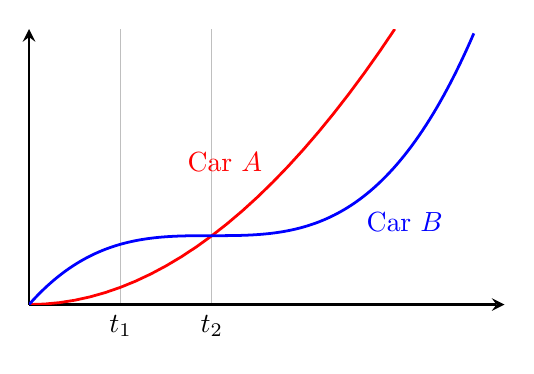
\begin{tikzpicture}
            \begin{axis}[
   	            xmin=0, xmax=2.6,
	            ymin=0, ymax=4,
	            major tick length={0},
	            xtick={0.5, 1},
	            ytick=\empty,
	            xticklabels={$t_1$, $t_2$},
            	line width=1pt, 
 	            axis lines=center, height=2 in, width=3 in, grid=major,
 	            restrict y to domain=0:4
	            ]
	            \addplot[red,domain=0:2] {x^2}
	            node [pos=0.5, above left] {Car $A$};
	            \addplot[blue,domain=0:4, samples=200] {(x-1)^3+1}
	            	 node [pos=0.5, below right] {Car $B$};
                \end{axis}
            \end{tikzpicture}
    	\end{center}

                  \item Suppose that a snowstorm begins at midnight, and the function $f(t)$ gives the depth of snow in inches on my driveway, where $t$ is the number of hours past midnight. Interpret the statements $f(2) = 3$ and $f'(3) = 2$ in the context of this problem.          
                 \item Consider the function $\displaystyle y=f(x) = \frac{1}{1+ce^{-x}}$.  Does this function satisfy the differential equation $y'=y(1-y)$?
                 \item In the study of probability and statistics, a function that describes the probabilities associated with a random number (more precisely, a ``random variable'') is called a ``cumulative distribution function'' (sometimes abbreviated c.d.f.) A cumulative distribution function $F(x)$ gives the probability that a random variable has a value less than or equal to $x$. Random variables are alternately defined by ``probability density functions,'' which indicate the relative probabilities of different outcomes. These two types of functions are related: the derivative of a cumulative distribution function is a probability density function. Below are two examples of graphs of cumulative distribution functions. Graph their corresponding probability density functions.
                 
 \tikzset{
    declare function={
        normcdf(\x,\m,\s)=1/(1 + exp(-0.07056*((\x-\m)/\s)^3 - 1.5976*(\x-\m)/\s));
    }
}
\begin{center}
\begin{tikzpicture}[]
\begin{axis}[%
  xlabel=$x$,
  ylabel=$F(x)$,
  domain=-3:3,
  grid=major
]
  \addplot [smooth, black] {normcdf(x,0,1)};
\end{axis}
\end{tikzpicture} 
\end{center}

\begin{center}
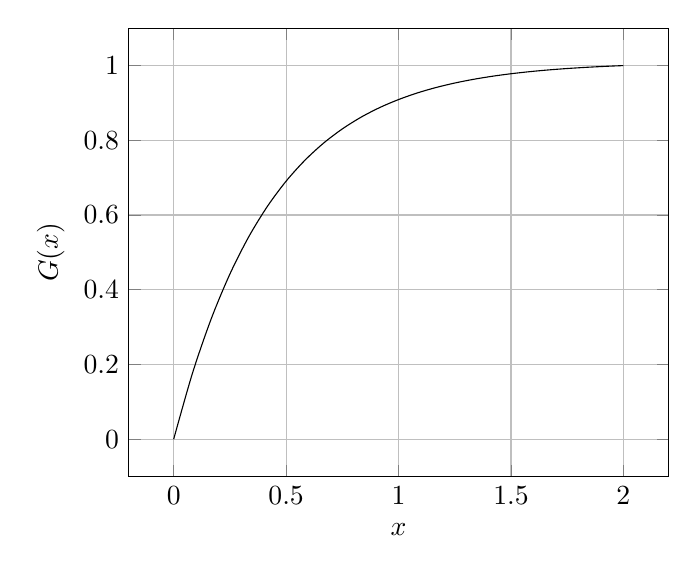
\begin{tikzpicture}[]
\begin{axis}[%
  xlabel=$x$,
  ylabel=$G(x)$,
  domain=0:2,
  grid=major
]
  \addplot [smooth, black, domain=0:2] {100/99*(1-10^(-x))};
\end{axis}
\end{tikzpicture} 
\end{center}
                  \item Find the derivative of each of the following functions. You should confirm all of your answers are correct using a computer algebra system (such as Wolfram Alpha). You should be able to compute derivatives such as these with 100\% accuracy.
                \begin{enumerate}
                    \item $\displaystyle f(x) = e^{x^2}$
                    \item $\displaystyle f(x) = (e^x)^2$
                    \item $\displaystyle f(t) = \log_{12}(5t)$
                    \item $\displaystyle f(x) = \frac{e^{bx}}{1+e^{bx}}$
                    \item $\displaystyle f(b) = \frac{e^{bx}}{1+e^{bx}}$
                    \item $\displaystyle f(x) = \ln{\left(\left(\sin{(1+x)}\right)^2e^{5x}x^{-2}(-2x^4+7x-8)\right)}$
                    
                    \item $\displaystyle f(x) = \frac{e^{x^2}}{\ln(x^2)}$
                    \item $\displaystyle f(x) = \ln(\sqrt{x})\cdot \sqrt{x}$
                    \item $\displaystyle f(x) = \frac{1}{4x^2}$
                    \item $\displaystyle f(\mu) = \frac{e^{-\mu}\mu^x}{x!}$
                \end{enumerate}
                \item Find the derivative of $\displaystyle f(x)=\prod_{k=1}^n (x_k-a)^k$. 
                \item Find the derivative of $\displaystyle f_k(x) = \sum_{n=0}^k \frac{x^n}{n!}$.
                \item Find the derivative of $\displaystyle f(x) = \sum_{n=0}^\infty \frac{x^n}{n!}$, assuming that you can differentiate an infinite sum term-wise. Compare the terms of $f'(x)$ to those of $f(x)$. Based on your observation, can you guess what function $f(x)$ is?
                \item Find derivative of $\displaystyle f(p) = \ln{\left(\prod_{i=1}^n p^{x_i}(1-p)^{1-x_i}\right)}$. Simplify using the laws of logarithms before differentiating. Note that the values $x_i$ should be treated as unknown constants, while $p$ is the variable of differentiation.
          
                
           
                \end{enumerate}

\end{document}
